\documentclass[a4paper,12pt]{article}
 
\usepackage[utf8]{inputenc}
\usepackage[francais]{babel}
\usepackage{graphicx}
\usepackage{amsmath}
\usepackage[font={small,it}]{caption}
\usepackage{setspace}
\usepackage{geometry}
\usepackage{multirow}
\usepackage{emp}
\usepackage{url}




\author{\textbf{Alexandre Nicaise}\\Master de Compétence Complémentaire en Informatique 2014-2015 \\Encadrant : Jean Meunier, Jean-Luc Mari, Arnaud Polette}
\title{\vfill \textbf{Application mobile : Visualisation 3D de la cornée}}
\date{\today\vfill}
\onehalfspacing
\geometry{hmargin=2.5cm,vmargin=1.5cm}
 
 
\begin{document}

\renewcommand{\tablename}{Tableau}

\begin{figure}
    \begin{minipage}[t]{6cm}
        
\includegraphics[width=4cm]{amu.png}
    \end{minipage}
    \begin{minipage}[t]{10cm}
    	\raggedleft
        
\includegraphics[width=4cm]{logoUDEM.png}
    \end{minipage}
\end{figure}


\maketitle

\thispagestyle{empty}



%%%%%%%%%%%%%%%%%%% Remerciement %%%%%%%%%%%%%%%%%%%%%%%%
\newpage
~
\vfill
\textbf{Remerciement}
\thispagestyle{empty}


Je voudrais remercier Jean Meunier, mon ma\^itre de stage, pour m'avoir accueilli au sein de son équipe à Montréal et pour m'avoir fait découvrir le monde de la vision. Je remercie Jean-Luc Marie, mon responsable de master, pour nous avoir transmis cette offre de stage et pour ces conseilles. Je remercie Sébastien Roy pour m'avoir fait découvrir VTK et pour ces conseilles en Android. Je remercie Arnaud Polette pour ces conseilles sur la partie de programmation, et de visualisation de la cornée. Je remercie aussi Rania pour m'avoir appris  à utiliser CMAKE. Je remercie toutes les personnes de la pièce 2384 pour leur accueille. Je remercie Annie Lebreton, ma conjointe pour ca relecture de mon rapport. Enfin, je remercie mes parents sans qui je n'aurais pas pu faire cette expérience.
\vfill

%%%%%%%%%%%%%%%%%%% sommaire %%%%%%%%%%%%%%%%%%%%%%%%%%%%%%
\newpage
\tableofcontents
\thispagestyle{empty}



%%%%%%%%%%%%%%%%%%% Introduction %%%%%%%%%%%%%%%%%%%%%%%%
\newpage
\setcounter{page}{1}
\pagestyle{plain}
\section{Introduction}
	\subsection{Département Informatique et Recherche Opérationnelle}
Fondé en 1966, le Département Informatique et Recherche Opérationnelle (DIRO) fut le premier département d’informatique créé au Québec et le troisième au Canada. Le DIRO est situé dans le pavillon André Aisenstadt qui fait partie de l'Université de Montréal (UdeM). L'UdeM a été fondée en 1978 et a été la première Université francophone de Montréal. Elle fait partie des quatre établissements supérieur de Montréal au Québec. Selon la firme QS (Quacquarelli Symonds), l'université de Montréal se classe au 33ieme rang des meilleures universités du monde en recherche opérationnelle. Elle fait également belle figure en informatique, prenant place parmi le groupe de tête constitué de 150 universités d'excellence. 
		
Durant ce stage, j'ai pu intégrer l'équipe du DIRO dirigé par Jean Meunier. Il s'intéresse à l'analyse et au traitement numérique d’images et de vidéos dans un contexte médical. Ici nous allons plutôt nous intéresser à l'œil et plus précisément à la cornée.

	\subsection{Contexte Biologique}
		\subsubsection{L'œil}
		
L'œil est l'organe de la vision, c'est à dire qu'il capte la lumière afin que le cerveau puisse l'analyser et ainsi interagir avec son environnement. Il possède trois membranes opaques (sclérotique, choroïde et rétinienne) et quatre milieux transparents (cornée, humeur aqueuse, cristallin et humeur vitrée) (Figure : \ref{oeil}). Il est aussi protégé par plusieurs structures annexes comme les paupières, les cils et les sourcils.

\begin{figure}[h]
	\centering
	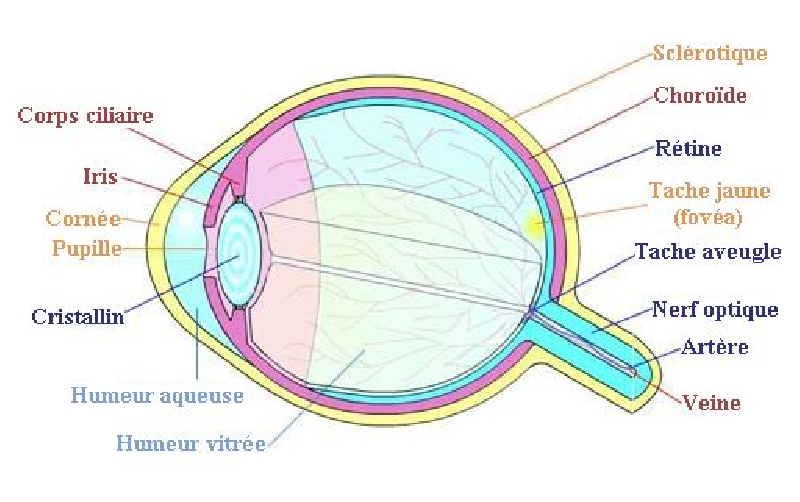
\includegraphics[width=15cm]{oeil.eps} 
	\caption{L'oeil (Gabrielle Bonnet et Gilles Camus) \cite{oeil1}}
	\label{oeil}
\end{figure}

L’œil est souvent comparé à un appareil photo. Il est constitué d'un système optique (un objectif) et d'une surface sensible à la lumière. Le système optique est constitué de la cornée et du cristallin. Il permet de capter les rayons lumineux provenant d'un objet source et de les dévier afin qu'ils convergent en un même point, idéalement situé dans le plan de la surface photosensible. Cette surface est située au sein de la rétine et est recouverte de cellules appelées photorécepteurs. Les photorécepteurs sont soit des cônes permettant la vision diurne, soit des bâtonnets permettant la vision nocturne. Ensuite nous quittons le domaine de l'appareil photo et passons dans le traitement de l'information. Les photorécepteurs créent un influx nerveux en réaction à leurs exposition aux rayons lumineux. L'influx nerveux passe dans le nerf optique pour atteindre l'aire visuelle du cerveau. Le cerveau se charge ensuite de déchiffrer l'information contenue dans l'influx nerveux afin de permettre l'interaction avec l'environnement. (Figure : \ref{fig:Vision})

\begin{figure}[h]
	\centering
	\includegraphics[height=10cm]{Vision.eps} 
	\caption{Présentation du mécanisme de la vision}
	\label{fig:Vision}
\end{figure}


Ici nous nous intéresserons plus à un des éléments du système optique : la cornée.



		\subsubsection{La cornée}

La cornée est un composant oculaire essentiel au fonctionnement de la vision: elle est la première structure que rencontre la lumière qui pénètre l’œil. Son rôle principal est de faire converger les rayons lumineux incidents vers le cristallin, avant de rencontrer la rétine et d'enclencher la cascade visuelle en créant l'influx nerveux. Cette convergence est représentée par le pouvoir optique de la cornée. Le pouvoir optique, aussi appelé pouvoir réfractif ou de vergence, représente le degré de réfraction des rayons lumineux lors de la traversé d'un milieu. Il est représenté par une unité de mesure appelée dioptrie et qui est une unité de vergence.  Une valeur négative montre une divergence alors qu'une valeur positive montre une convergence. La cornée assure les deux tiers du pouvoir optique des structures oculaires, le tiers restant étant dévolu au cristallin. \cite{bookGatinel, gatinel}
\vspace{0.15cm}

\parindent=0em
Le pouvoir optique supérieur de la cornée par rapport à la rétine découle des éléments suivants : \vspace{0.15cm}
\begin{itemize}\setlength{\itemsep}{1mm}
	\item[$\bullet$] une courbure plus importante que celle du cristallin non accommodé. Les accommodations du cristallin sont des modifications effectuées sur celle-ci afin de modifier la réfraction du cristallin et ainsi améliorer la netteté de l'image.
	\item[$\bullet$] le contact avec l'air ambiant, offrant la plus grande différence d'indice de réfraction aux rayons lumineux incidents par rapport au cristallin qui est au contact d'un liquide et donc avec un indice de réfraction moindre. 
\end{itemize}
\parindent=1.5em

 \vspace{0.5cm}
La cornée est un tissu non vascularisé et transparent. C'est une coupole hémisphérique au contact direct de l'air. Elle couvre environ un cinquième de la surface de l’œil et a un diamètre d'environ 12 mm. La cornée est légèrement plus épaisse en périphérie (0.6 mm) par rapport à son centre (0.5 mm). Pour qualifier l'épaisseur, j'utiliserai le terme de pachymétrie. Le rayon de courbure est d'environ 6.5 mm pour la surface postérieure et varie de 7 à 9 mm pour la surface antérieure. La transparence de la cornée et la régularité de la courbure permettent une transmission sans perte préjudiciable en quantité et qualité de l'information lumineuse. Seulement 4\% à 6\% de la lumière incidente est réfléchie par la surface cornéenne. Cette propriété de réflexion est mise à profit pour la réalisation de l'examen de topographie cornéenne.\cite{gatinel}

\begin{figure}[h]
	\centering
	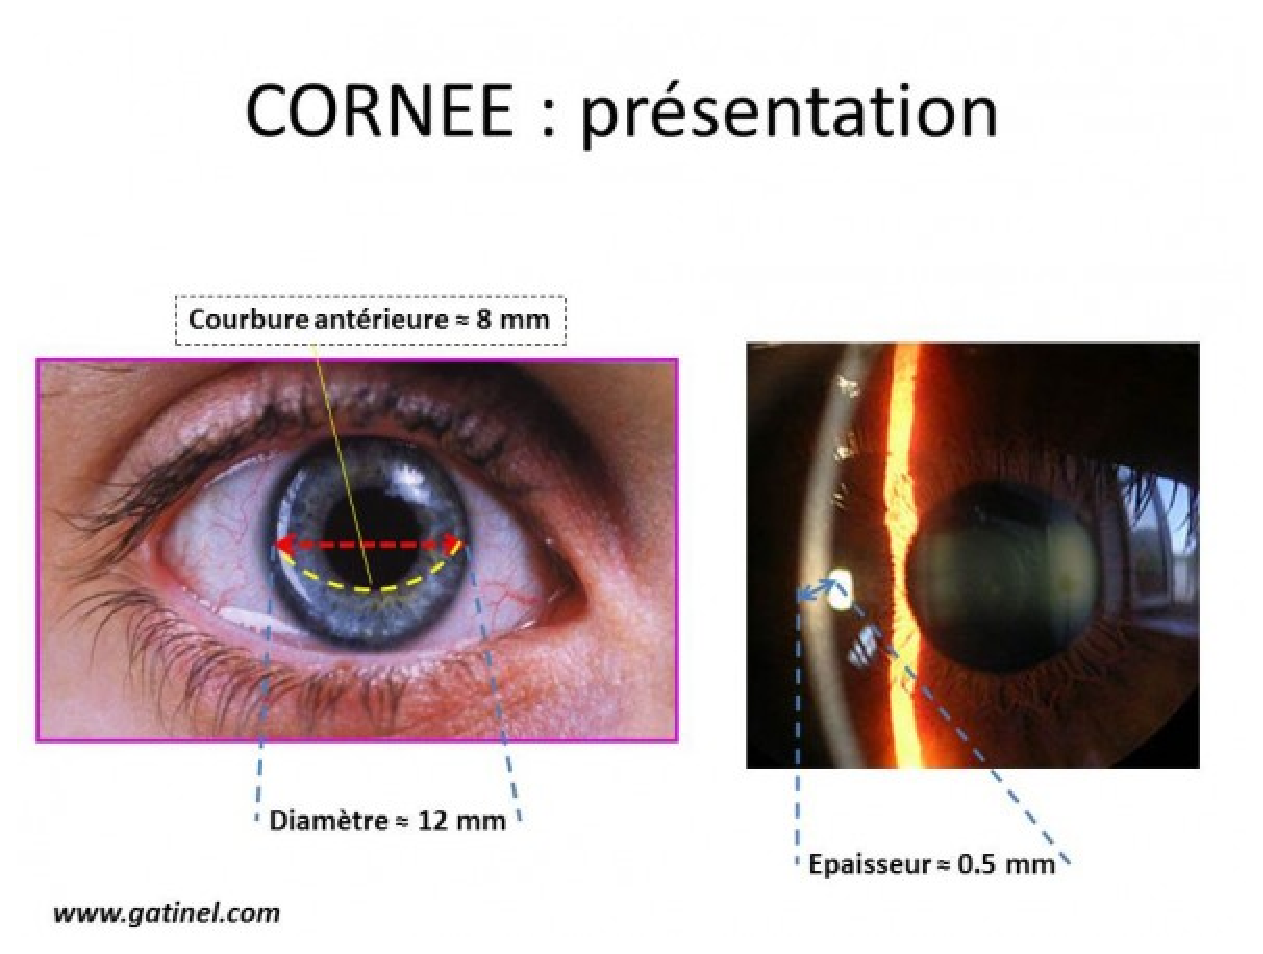
\includegraphics[width=16cm, trim=0cm 0cm 0cm 3cm, clip]{CorneePresentation.eps} 
	\caption{Présentation de la cornée. L'image de gauche montre le diamètre et la courbure moyenne de la cornée. L'image de droite montre l'épaisseur entre la surface antérieure et la surface postérieure aussi appelé pachymétrie.\cite{gatinel}}
\end{figure}


		\subsubsection{Topographie de la cornée}
La topographie permet de recueillir des informations relatives à la courbure ou au relief (élévation) de la cornée, grâce à la projection et l'analyse du reflet d'un motif lumineux éclairant ou balayant la cornée. Les images recueillies sont analysées de façon automatisée et des cartes en couleurs sont fournies au praticien pour interprétation. La topographie est courante lors d'un examen ophtalmologique, pour réaliser un diagnostic ou un suivi. En effet, des déformations peuvent être liées par exemple, à des pathologies, des traumatismes, une chirurgie, ou simplement à l'âge. Dès lors, la possibilité d'estimer et de caractériser cette déformation permet d'apporter une information pertinente au médecin pour aider son diagnostic.\cite{gatinel, arnaud}

Lors de mon stage, j'ai utilisé des données obtenues via l'appareil Orbscan II (Figure \ref{orbscan}) qui permet de mesurer l'élévation de la cornée. Il est capable de mesurer la partie antérieure ainsi que la partie postérieure de la cornée avec une marge d'erreur de l'ordre du micron. Les données peuvent se présenter sous la forme d'une grille 101x101 contenant les valeurs d'élévation qui ont été prises toute les 0.1 mm. A partir de cette matrice d'élévation, il est possible de construire des maillages qui seront utilisés par la suite pour la visualisation en 3 dimensions de la cornée. 

La cornée étant presque sphérique, un moyen simple et efficace de visualiser l'aspect de sa surface est d'utiliser une référence sphérique afin d'observer les différences entre la référence et la cornée. 
\vspace{0.25cm}

\begin{figure}[h]
	\centering
	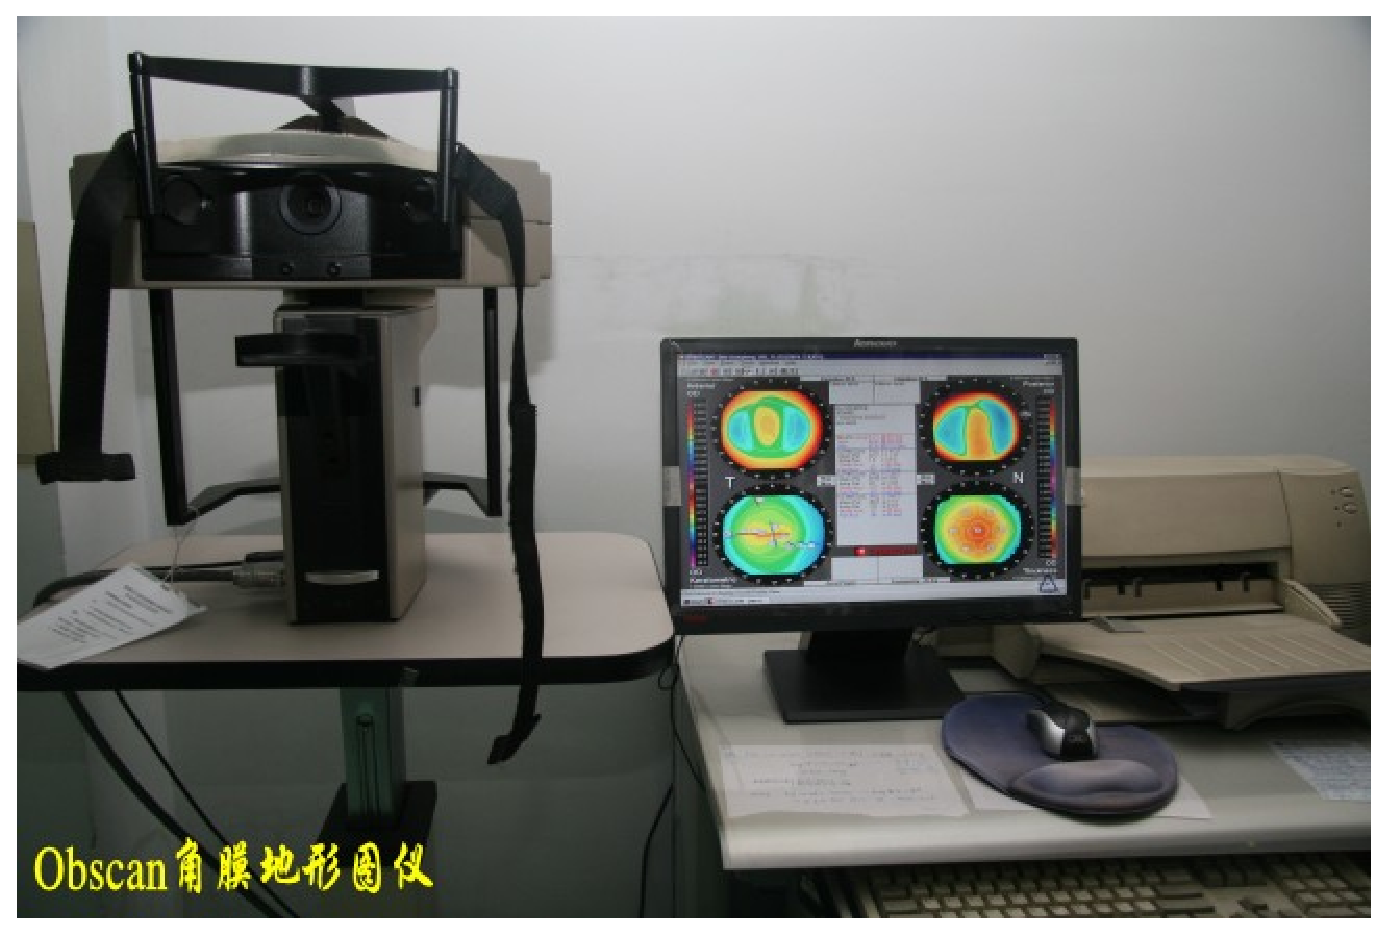
\includegraphics[ width=10cm]{Obscan.eps}
	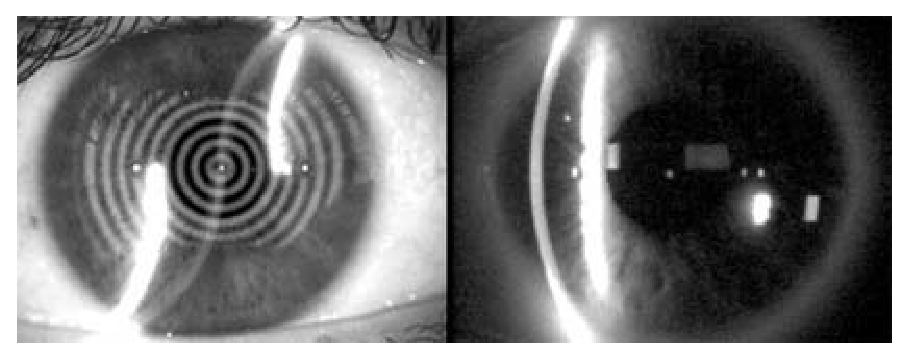
\includegraphics[width=10cm]{orbscanPrincipes.eps} 
	\caption{Orbscan II. L'image du dessus présente l'appareil. Les autres images présentent le principe de l'orbscan. Il associe la réflexion du disque de Placido (à droite) sur la cornée au balayage de l'œil par une fente lumineuse (à gauche).}
	\label{orbscan}
\end{figure}

\subsubsection{"Best Fit Sphere" (BFS)}

Afin d'affiner leurs diagnostics les praticiens ont besoin de mieux connaître l'aspect de la surface de la cornée. La cornée étant presque sphérique, il est possible de la comparer en faisant la différence des deux. Pour cela, on calcule la "Best Fit Sphere" (BFS) qui est la sphère qui correspond le mieux à la matrice d'élévation, puis on effectue la différence entre les deux surfaces. Cette différence va permettre de construire une carte semblable à celles utilisées par les géologues pour représenter les reliefs de la terre. En effet, afin de mettre en évidence ces "reliefs" ces différences sont représentées selon un jeu de couleur standard. Les différences positives seront associées à des couleurs chaudes (points à l'extérieur de la BFS) et les différences négatives (points à l'intérieur de la BFS) à des couleurs froides. Il est nécessaire de calculer deux BFS différentes, une pour la face antérieure et une pour la face postérieure. 
\vspace{0.5cm}

La BFS est calculée en minimisant la somme des distances au carré entre la sphère et chaque point de la cornée, ce qui donne l'expression suivante à minimiser :
\vspace{0.25cm}

$ f(c,R) = \overset{n}{\underset{k=1}{\sum}} \sqrt{(x_k-x_c)^2 + (y_k-y_c)^2 + (z_k-z_c)^ 2} - R^2$
\vspace{0.25cm}

Avec k un point de la cornée, c le centre de la BFS, R son rayon et n le nombre de point de la cornée.\cite{arnaud}

\vspace{0.25cm}
L'association d'image représentée par la figure~\ref{fig:CorneaConstruct} permet la visualisation des différentes étapes de construction de la carte topographique de la cornée. 

\begin{figure}[h]
	\centering
	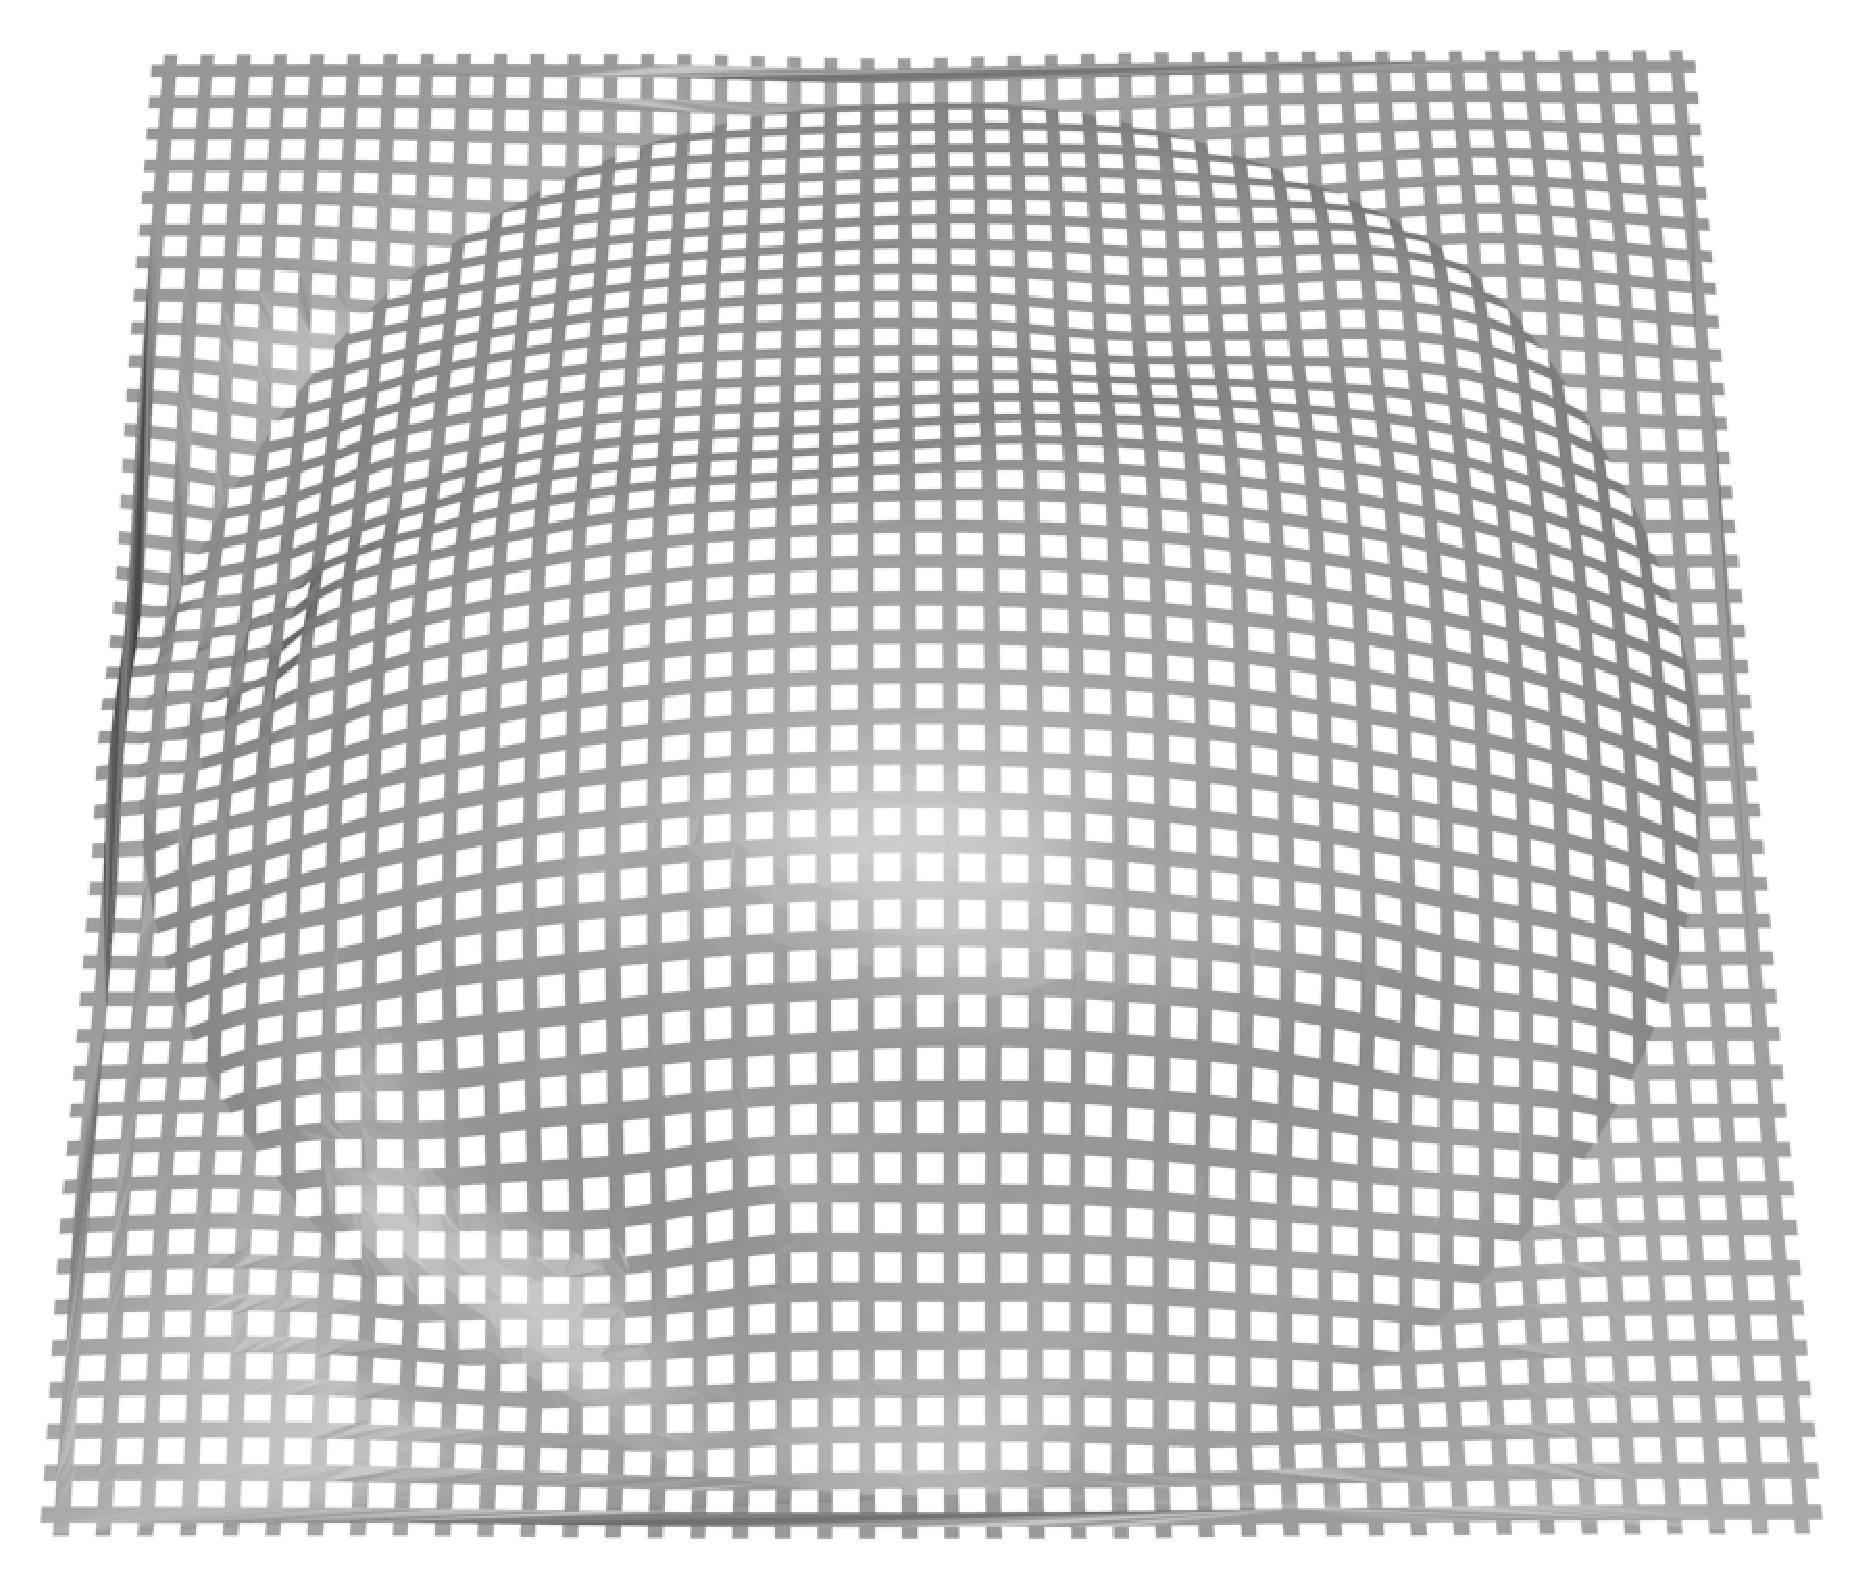
\includegraphics[ width=4cm]{bfs.eps}
	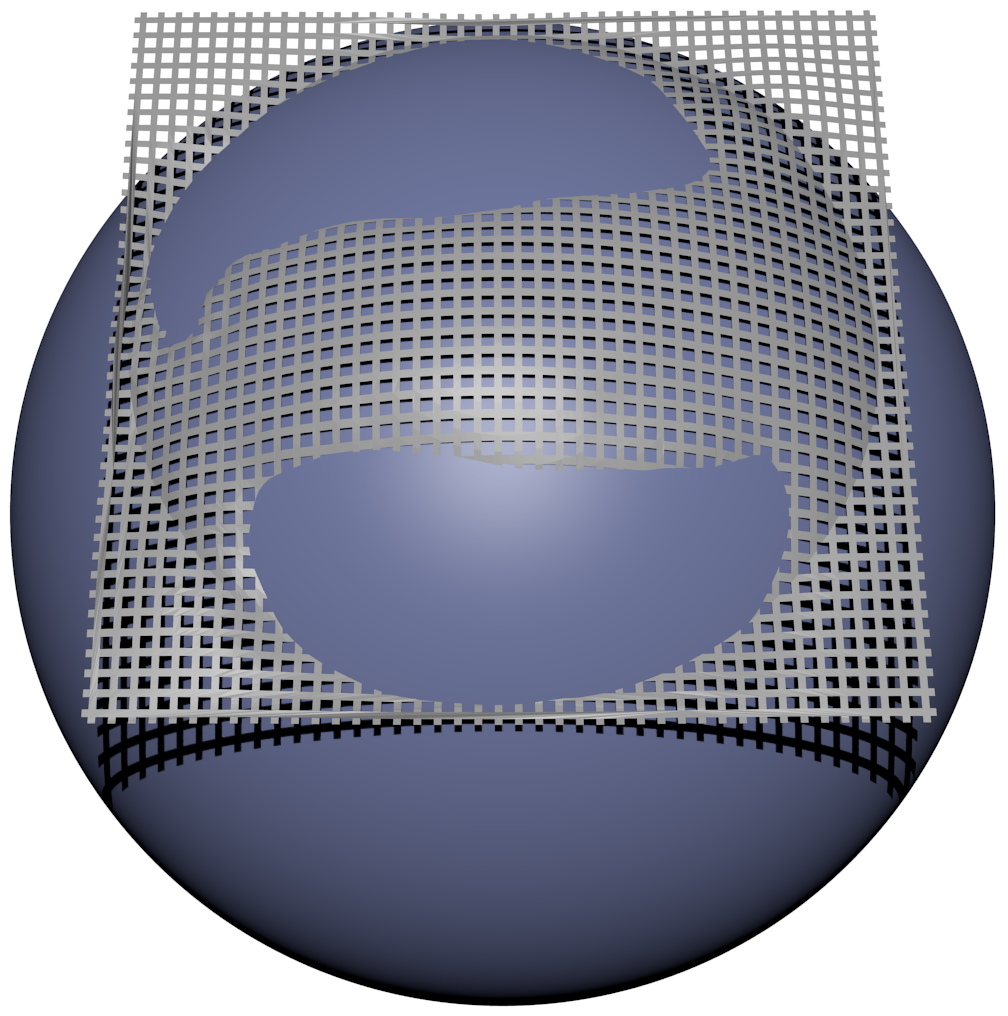
\includegraphics[ width=4cm]{carteElevation.eps}
	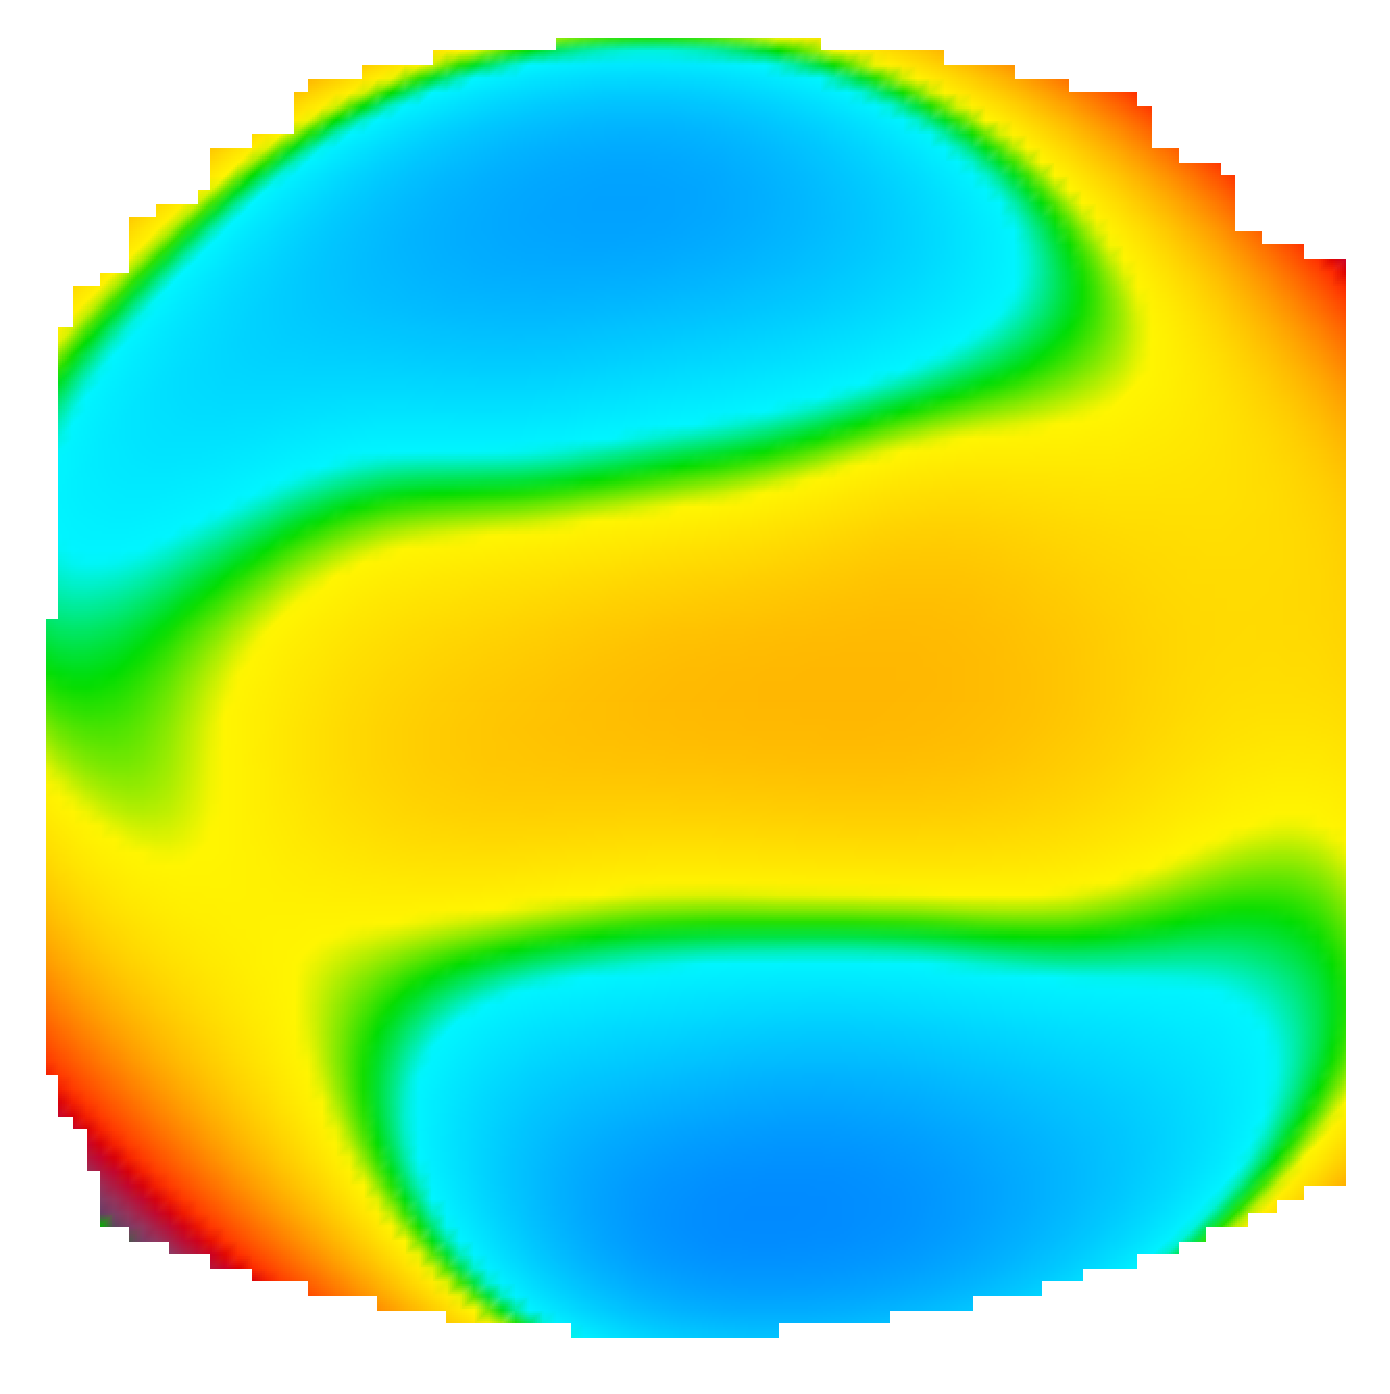
\includegraphics[ width=4cm]{carteElevationcouleur.eps}
	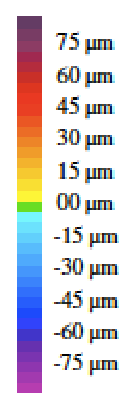
\includegraphics[ height=4cm]{pallette.eps}
	\caption{Présentation de la construction de la carte de couleur d'une cornée. A gauche nous pouvons voir la matrice 101x101 obtenue par l'orbscan. L'image suivante est la superposition de la BFS (Best Fit Sphere) et de cette matrice. La troisième image est l'ajout des couleurs afin de visualiser les relief de la cornée selon une palette de couleur située juste à côté. On peut voir que les couleurs froides sont situées en-dessous de la BFS, les couleurs chaudes au-dessus et le vert symbolise le passage à 0. \cite{arnaud}}
	\label{fig:CorneaConstruct}
\end{figure} 


\newpage
	\subsection{Problématique du stage}
Le but de mon stage a été de construire une application mobile permettant de visualiser une cornée en trois dimensions. Ce projet intéresse beaucoup les praticiens de l'hôpital, car cela faciliterait l'accès aux cartes topographiques des cornées de leurs patients. Ce projet a été débuté l'année dernière par Ouri Saban un étudiant du master CCI. Pour construire son application, il a utilisé Unity qui est une plateforme de développement permettant de construire des jeux vidéos. Le problème était que Unity ne possède pas de bibliothèque aloué à la visualisation scientifique. C'est pourquoi, j'ai repris le projet mais en utilisant du C++ afin d'utiliser la bibliothèque appelée Visual Tool Kit (VTK) permettant la visualisation scientifique. Mon stage contient donc 2 grandes partie : la visualisation de la cornée avec VTK en local et le portage de VTK sur Android. 

%%%%%%%%%%%%%%%%%%%%%%%%%%%%%%%%%%%%%%%%%%%% Math Meth %%%%%%%%%%%%%%%%%%%%%%%%%%%%%%%%%%%%%%%%%%%%%

\newpage
\section{Matériels et méthodes}
	\subsection{Données disponibles}
Pour mes tests, je me suis servi d'un document texte fournis par Arnaud Polette qui contient toutes les informations de la cornée obtenues par le biais de l'Orbscan. Elles sont sous la forme de plusieurs matrices 101x101 contenant les valeurs d'élévations et dont les valeurs de X et de Y sont situées de -5 à +5 mm séparées par des pas de 0.1 mm. Ces matrices ne sont pas complètement remplis par des valeurs d'élévation mais contiennent aussi des valeurs null.

\vspace{0.25cm}
\parindent=0em Ces matrices permettent de visualiser : %empêche l'espace avant le nouveau paragraphe
\begin{itemize}\setlength{\itemsep}{1mm}
	\item[$\bullet$] la face postérieure 
	\item[$\bullet$] la face antérieure
	\item[$\bullet$] la différence entre la postérieure et la BFS
	\item[$\bullet$] la différence entre la antérieure et la BFS
	\item[$\bullet$] la pachymetrie
	\item[$\bullet$] la courbure de la face antérieure
	\item[$\bullet$] la courbure de la face postérieure
\end{itemize}

\vspace{0.25cm}
\parindent=1.5em
 Pour réaliser la visualisation en 3D de la cornée, je me suis servi des matrices représentant la face antérieure, la face postérieure, la BFS et la pachymetry. Les rayons et centres des sphères utilisées sont déduites de ces matrices. Nous avons donc tout les éléments nécessaire à la visualisation en trois dimension de la cornée.

	\subsection{VTK (Visualisation Toll Kit)}
		\subsection{Généralité}
	 VTK est très utilisé par les chercheurs et permet l'infographie en trois dimension, le traitement d'image et la visualisation. C'est une librairie construite par Kitware qui est constituée de classes en C++ avec plusieurs couches de surfaces interprétées incluant le Tcl/Tk, Java et Python. Il utilise OpenGL qui permet la déclarer la géométrie d'objets sous forme de points, de vecteurs, de polygones, de bitmaps et de textures \cite{vtk}. OpenGL (Open Graphics Library) effectue ensuite des calculs de projection en vue de déterminer l'image à l'écran, en tenant compte de la distance, de l'orientation, des ombres, de la transparence et du cadrage. Nous avons choisi VTK car nous avons été séduits par une application open-source utilisant VTK appelé KIWIVIEWER qui fonctionne aussi bien sur Android, que sur iOS. De plus, VTK possède de nombreux exemples qui permettent d'apprendre à l'utiliser. Pour installer VTK, je clone le projet stocker sur github et je le compile via CMAKE (cf 2.4.2).

	 
		\subsubsection{Liste des fonctions utilisées}
\parindent=0em Pour la visualisation j'ai utilisé les éléments de vtk suivants :
\vspace{0.25cm}

\textbf{vtkPoints}	: stocke les coordonnées obtenues par le biais des matrices d'élévation 
\vspace{0.25cm}

\textbf{vtkFloatArray} : affecte un "scalar" à une coordonnée. Un scalar est une valeur qui permettra la représentation sous forme de couleurs. Ici nous utiliserons les valeurs d'élévations.
\vspace{0.15cm}

\textbf{vtkCellArray}  : construit le maillage. Le maillage est la représentation d'une surface (ici la cornée) en la subdivisant en un ensemble de polygones. Il est composé de sommets,  connectés les uns aux autres par des faces ou facettes de forme polygonale. Lorsque toutes les faces sont des triangles, on parle de maillage triangulaire (trimesh), ou de triangulation selon les domaines. Les maillages par quadrilatères sont aussi très courants. En trois dimensions, il est aussi possible d'utiliser des maillages volumiques, qui relient les sommets par des tétraèdres, des hexaèdres et des prismes (tableau \ref{matriceElev} et figure \ref{fig:maillage}). Ici, j'ai utilisé le maillage triangulaire. 

\begin{table}[h]
	\centering
	\begin{tabular}{cccccc}
		1.05 & 1.20 & 1.25 & 1.20 & 1.05  \\
		1.20 & 1.35 & 1.40 & 1.35 & 1.20 \\
		1.25 & 1.40 & 1.45 & 1.40 & 1.25 \\
		1.20 & 1.35 & 1.40 & 1.35 & 1.20 \\
		1.05 & 1.20 & 1.25 & 1.20 & 1.05 
	\end{tabular}
	\caption{matrice d'élévation obtenue via l'Orbscan}
	\label{matriceElev}
\end{table}


\begin{figure}[h]
	\centering
	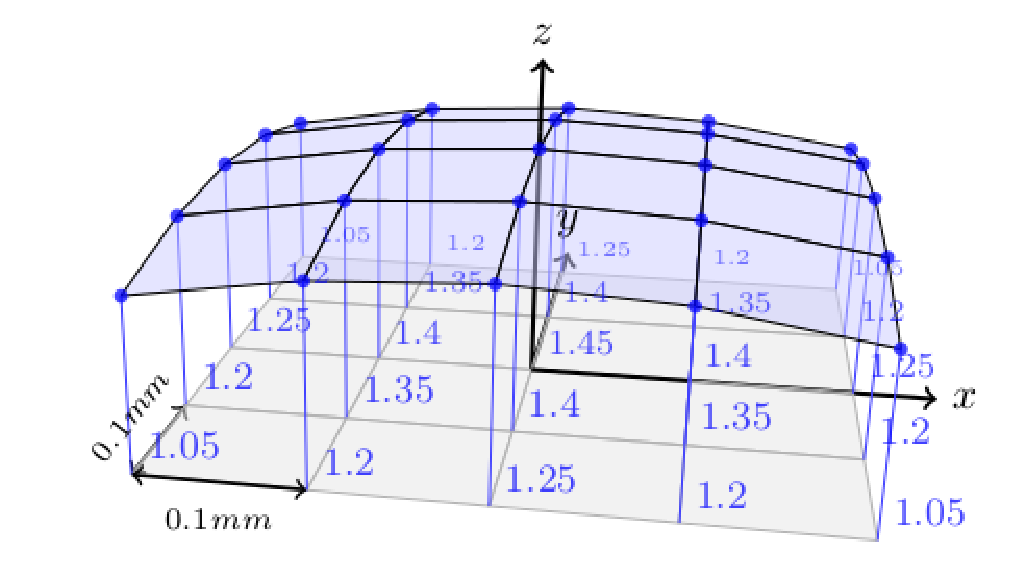
\includegraphics[width=10cm]{maillage.eps}  
	\caption{Maillage a partir de la matrice d'élévation du Tableau \ref{matriceElev} \cite{arnaud}. }
	\label{fig:maillage}
\end{figure} 

\vspace{0.25cm}

\textbf{vtkPolyData} : regroupe les objets vtkPoints, vtkFloatArray et vtkCellArray.
\vspace{0.25cm}

\textbf{vtkPolyMapper} 	: permet la transformation de la structure de données contenues dans vtkPolyData en primitives OpenGL. Les primitives OpenGL sont des points, des lignes ou des triangles. Il permet aussi l'association de couleurs qui peuvent être contrôlées en spécifiant une table de couleurs (lookup table) et un intervalle.
\vspace{0.25cm}

\textbf{vtkLookupTable}  : permet de spécifier la table de couleur utilisé pour la visualisation.
\vspace{0.25cm}

\textbf{vtkScalarBarActor} : permet d'afficher une barre dans la fenêtre représentant la pallette de couleur contenue dans vtkLookupTable.
\vspace{0.25cm}

\textbf{vtkActor} : sert à positionner et orienter l'objet, à le colorer et choisir des propriétés graphiques. 
\vspace{0.25cm}

\textbf{vtkRenderer} : lance les algorithmes nécessaires au rendu de l'objet.
\vspace{0.25cm}

\textbf{vtkRenderWindow} : spécifie une fenêtre qui affiche le rendu.
\vspace{0.25cm}

\textbf{vtkRenderWindowInteractor} : permet l'intéraction avec l'objet en faisant bouger la caméra.

 \vspace{0.25cm}
La figure~\ref{fig:VTKMeth} permet de visualiser la construction de la carte d'élévation (mapper) avec VTK à partir d'une matrice d'élévation (exemple tableau \ref{matriceElev}).

 \vspace{0.25cm}
Pour utiliser VTK, nous pouvons utiliser plusieurs langage tel que le java, le python, le C, le C\# ou encore le C++. Étant donné que les exemples mis à disposition pour Android sont codé en C++, j'ai donc utilisé ce langage afin de créer mon propre programme.




\begin{figure}[h]
	\centering
	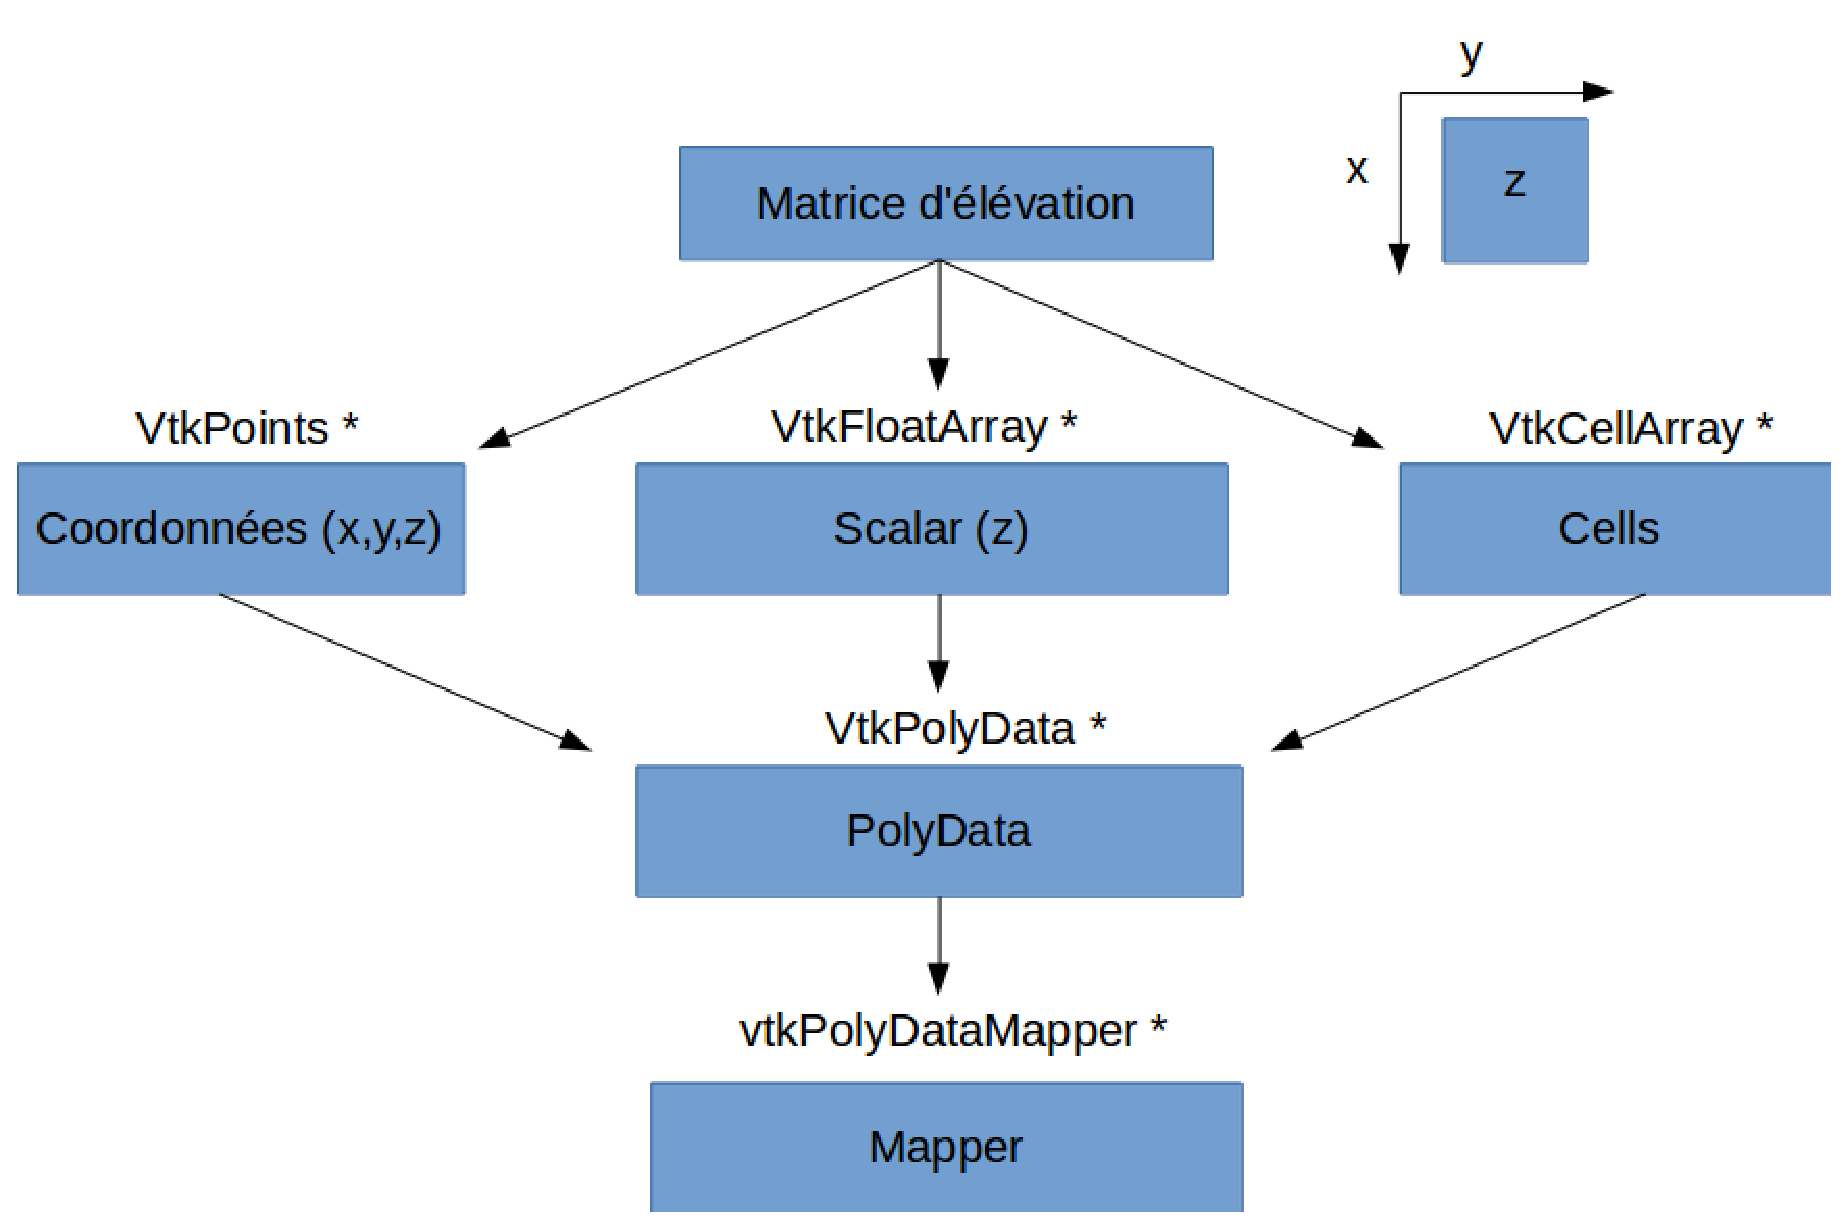
\includegraphics[width=15cm]{VTKMeth.eps}  
	\caption{Construction de l'objet polydataMapper à partir d'une matrice d'élévation. Un schéma de la matrice est représenté en haut à droite de la figure. A partir de cette matrice trois éléments sont extraits : les coordonnées qui sont stockées dans un vtkPoints, les valeurs d'élévations qui sont associées à une couleur stockée dans un vtkFloatArray et les cellules qui représentent le maillage dans un vtkCellArray. Ces trois éléments sont ensuite associés dans un vtkPolyData qui servira ensuite à construire le mapper.}
	\label{fig:VTKMeth}
\end{figure} 

	\subsection{Langage de programmation : C++}	
		\subsubsection{Généralité}
\parindent=1.5em
	Le C++, descendant du C, est un langage de programmation compilé apparu en 1983 et ayant subit plusieurs révisions depuis, dont la dernière était en 2014. Avec lui, nous pouvons programmer sous les paradigmes : 
	\parindent=0em
	
\vspace{0.25cm}
\textbf{Procédurale} : qui permet de décomposer le code en sous fonctions pouvant être réutilisées plusieurs fois dans le programme voir s'appeler elles-même (récursivité)

\vspace{0.25cm}
\textbf{Orienté objet} : permet l'utilisation des objets qui sont des ensembles groupé de variables et de méthodes associées à des entités intégrant naturellement ces variables et méthodes. Elle est organisé en classes, possédant des constructeurs permettant d'instancier l'objet, des destructeurs permettant de le détruire et les différentes méthodes (fonctions).

\vspace{0.25cm}
\textbf{Générique} : permet la définition d'algorithmes identiques opérant sur des données de types différents.
\parindent=1.5em
\vspace{0.25cm}

 		\subsubsection{Programmation}

  Pour coder sous ce langage plusieurs choix étaient à ma disposition : un environnement de développement (IDE) ou l'association entre un éditeur de texte et CMAKE (Cross platforme MAKE). 
  
  Dans un premier temps, j'ai utilisé un IDE (code::block) qui est un ensemble d'outils permettant de faciliter le travail du développeur. Il possède donc un éditeur de texte destiné à la programmation, des fonctions permettant de démarrer le compilateur ou l'éditeur de liens par simple pression sur un bouton et un débogueur en ligne. Le débogueur en ligne permet d'exécuter le programme en construction ligne par ligne. 
  
  Dans un deuxième temps, j'ai utilisé un éditeur de texte (Sublime text) couplé à CMAKE. Sublime text est un éditeur de texte conçu pour la programmation et CMAKE est un logiciel de compilation multiplateforme. CMAKE va utiliser des fichiers appelés "CMAKELists.txt", communs pour toutes les plateformes, afin de générer des makefiles. Les makefiles sont utilisés par le programme make pour exécuter un ensemble d'actions, comme la compilation d'un projet, l'archivage de document, la mise à jour de site, etc ... Ici on l'utilise pour la compilation du projet en C++.
 
\vspace{0.25cm}
\parindent=0em
  Mon projet s'organise de la manière suivante : 
  
\textbf{main.cpp} :  fichier contenant la fonction "main" qui marque le début du programme. Elle est appelé par le système d'exploitation et ne peut pas être appelé par le programme, c'est-à-dire qu'elle ne peut pas être récursive.
 
\textbf{header} : dossier qui contient les "header", c'est-à-dire des fichiers définissant les classes que j'ai construit et contenant leurs prototypes.
 
\textbf{src} : dossier qui contient les fichiers qui implémente les classes défini dans le dossier header. 

\textbf{build} : dossier où le projet a été compilé avec CMAKE.
\parindent=1.5em




	%%%%%%%%%%%%%%%%%%%%%%%%%%%%%%%%% Résultat %%%%%%%%%%%%%%%%%%%%%%%%%%%%%%%%%%%%%%%%%%%%%%%%%%%%%%%%%%


\newpage
\section{Résultat}
	\subsection{Les classes}
Le C++ étant un langage de programmation orienté objet, j'ai pu créer plusieurs classes aidant à l'organisation de mon code. Je vais vous présenter les différentes classes ainsi que leurs diagrammes UML.  

\vspace{0.25cm}
Tout d'abord, nous avons les classes représentant les données de la cornée : DataCornee, et ParserTopos.
\parindent=0em

\vspace{0.25cm}
\textbf{DataCornee : (figure : \ref{DataCornee})}

Elle représente les données d'une cornée en leur donnant un nom, comme "Surface anterior", et avec un tableau en deux dimensions contenant les données d'élévation de la cornée. Des fonctions retournent le nom et le tableau en deux dimensions permettant ainsi de le réutilisé dans le programme.

\begin{figure}[h]
\centering
	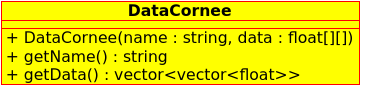
\includegraphics[width=8cm]{DataCornee.png} 
	\caption{Diagramme UML de la classe DataCornee.}
	\label{DataCornee}
\end{figure}

\textbf{ParserTopos : }

Cet objet représente les données contenues dans un fichier de référence grâce à une liste d'objets "DataCornee". Chaque matrice de données peut être appelée séparément grâce à des méthodes. Cet objet contient les rayons des sphères utilisées pour calculer la BFS et les coordonnées de leurs centres respectifs. Il stocke aussi les coordonnées réelles utilisées en x et en y (de -5 à 5mm par pas de 0.1mm). 

\begin{figure}[h]
\centering
	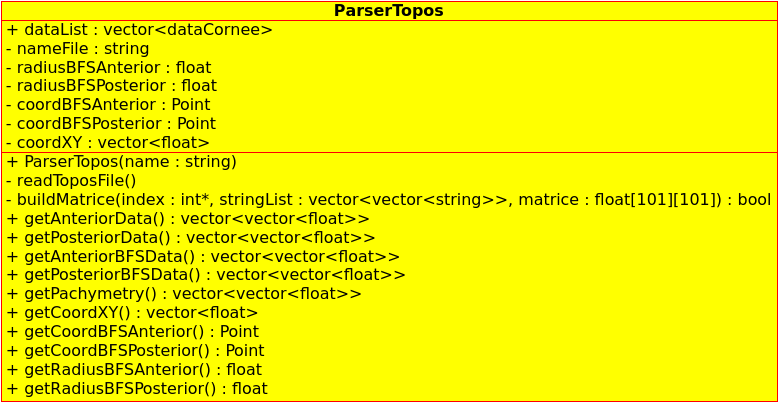
\includegraphics[width=15cm]{ParserTopos.png} 
	\caption{Diagramme UML de la classe ParserTopos.}
\end{figure}



%\textbf{DataPachymetry : } 
%reprend les données contenues dans topos afin de reconstruire les données de la pachymétrie. Pour cela, je lui donne soit deux matrices représentant les surfaces antérieures et postérieures de la cornée soit l'objet ParserTopos. Il construit ensuite la matrice de coordonnée qui sera utilisée dans la visualisation de la pachymétrie. Nous verrons cela un peu plus tard.

\vspace{0.25cm}
\parindent=1.5em
Ensuite, nous avons les classes permettant la visualisation de la cornée en utilisant VTK : ColorElevationMap, SurfaceElevationMatrice, SurfaceScalarElevationFromMatrice, PachymetryVisualisation, PachymetryVisualisationFromMatrice, VolumeVisualisation.
\parindent=0em

\textbf{ColorElevationMap : }
permet de stocker les objets VTK utilisés pour la visualisation (vtkPoints, vtkCellArray, vtkFloatArray, vtkPolydata, vtkPolyDataMapper, vtkActor). Elle contient aussi les méthodes nécessaires à la construction des cellules utilisées dans le maillage. Cette classe est la principale, c'est à dire qu'elle sera héritée par les autres classes utilisant VTK.

\begin{figure}[h]
	\centering
	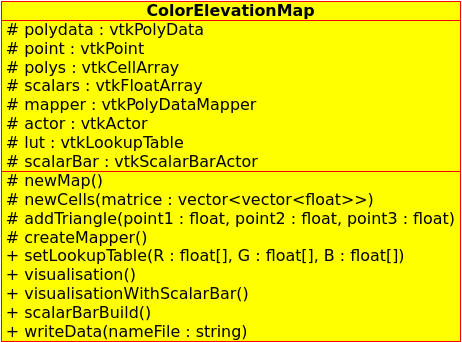
\includegraphics[width=10cm]{ColorElevationMap.png} 
	\caption{Diagramme UML de la classe ColorElevationMap}
\end{figure}

\textbf{SurfaceElevationFromMatrice : }
hérite de ColorElevationMap, elle permet la visualisation d'une surface via une matrice d'élévation (surface antérieure ou postérieure de la cornée). Dans cette classe, on ajoute des méthodes permettant d'extraire les coordonnées et les "scalars" à partir d'une matrice car celles-ci ne sont pas présentes dans ColorElevationMap.

\begin{figure}[h]
	\centering
	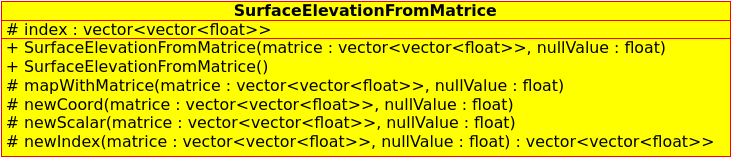
\includegraphics[width=15cm]{SurfaceElevationFromMatrice.png} 
	\caption{Diagramme UML de la classe SurfaceElevationFromMatrice}
\end{figure}


\textbf{SurfaceScalarFromMatrice : }
hérite de SurfaceElevationFromMatrice, elle permet la visualisation d'une surface via 2 deux matrices. La première est une matrice d'élévation, la deuxième représente les valeurs des différences entre la BFS et sa surface associée. Dans cette classe, j'ai fais en sorte d'adapter une des méthodes de la classe héritée afin qu'elle prenne en compte les deux matrices au lieu d'une.

\begin{figure}[h]
	\centering
	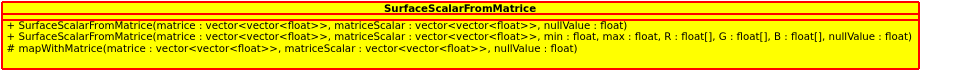
\includegraphics[width=18cm]{SurfaceScalarFromMatrice.png} 
	\caption{Diagramme UML de la classe SurfaceScalarFromMatrice}
\end{figure}

\textbf{VolumeVisualisation : }
hérite de ColorElevationMap, elle permet de créer un objet de VTK permettant de donner une impression de volume. Dans cette classe on ajoute toutes les méthodes nécessaires à la construction du volume (cf:plus loin).

\begin{figure}[h]
	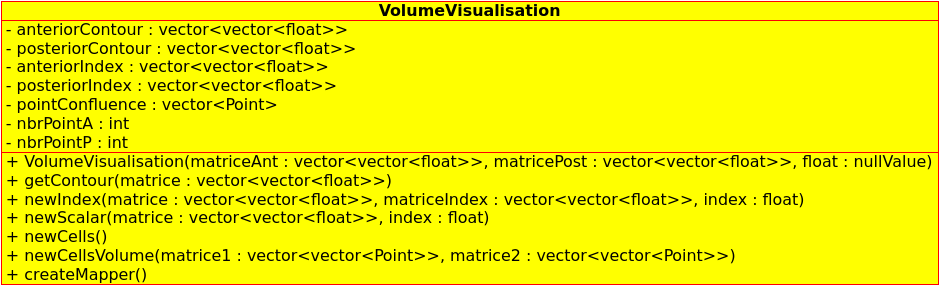
\includegraphics[width=18cm]{VolumeVisualisation.png} 
	\caption{Diagramme UML de la classe VolumeVisualisation}
\end{figure}

%\textbf{PachymetryVisualisation : }
%hérite de ColorElevationMap, elle permet de visualiser les données de l'objet DataPachymetry.

%\textbf{PachymetryVisualisationFromMatrice : }
%hérite de ColorElevationMap, permet de visualiser la pachymétrie de la cornée contenue dans un objet ParserTopos.

\begin{figure}[h!]
	\centering
	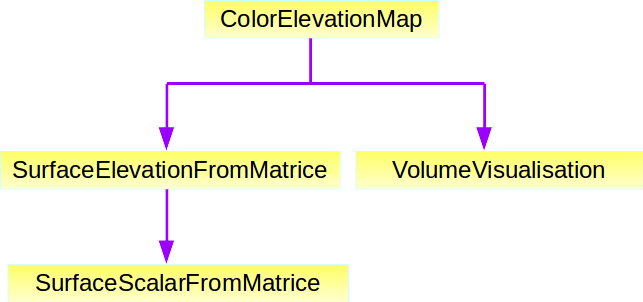
\includegraphics[width=15cm]{heritage.png} 
	\caption{Héritage}
\end{figure}



\vspace{0.25cm}
\parindent=1.5em

 J'ai aussi créé d'autres classes dont certaines représentent des notions tel que les points, les triangles ou encore les vecteurs. Les autres classes ne représentent pas des objets mais contiennent un ensemble de méthodes utiles dans certains cas. Par exemple, j'ai construit une classe contenant l'ensemble de mes fonctions qui permettent de traiter des variables de type string.
 
	\subsection{Visualisation des faces antérieure et postérieure}
	Grâce à VTK j'ai donc pu visualiser les faces antérieure (figure : \ref{AntScalarBar}) et postérieure (figure \ref{PostScalarBar}). Les couleurs utilisées correspondent à la différence entre la cornée et la BFS et sont utilisées par les praticiens. Les couleurs peuvent \^etre visualisées sur une palette sur la figure \ref{AntScalarBar}. Ensuite j'ai pu associer les deux faces dans une m\^eme fen\^etre (figure \ref{FaceAntPost}).
	
\begin{figure}[h!]
	\centering
	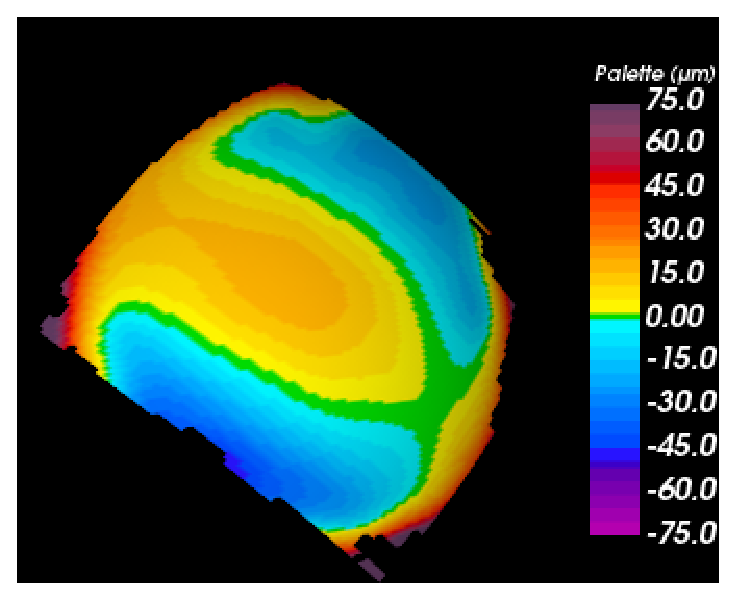
\includegraphics[width=10cm]{AntScalarBar.eps} 
	\caption{Face antérieure de la cornée}
	\label{AntScalarBar}
	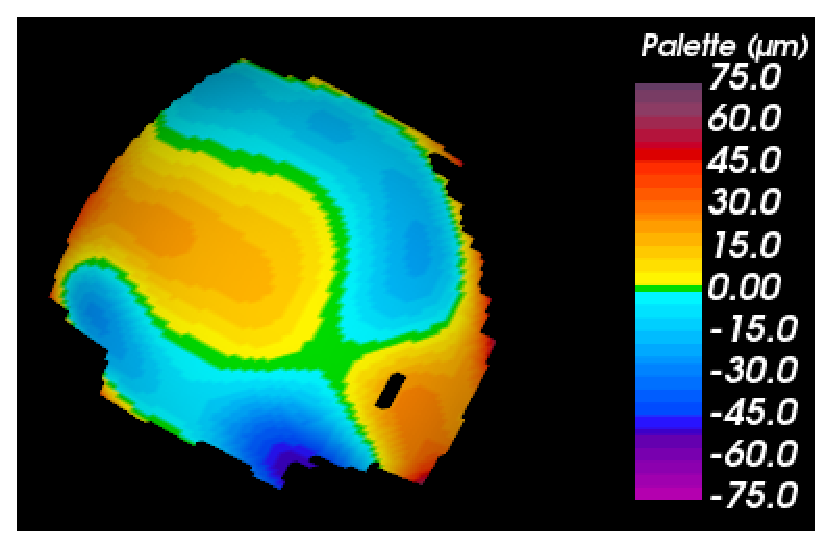
\includegraphics[width=10cm]{PostScalarBar.eps} 
	\caption{Face postérieure de la cornée}
	\label{PostScalarBar}
	
\includegraphics[width=10cm]{FaceAntPost.eps} 
	\caption{Face antérieur (au-dessus) et face postérieur (en-dessous)}
	\label{FaceAntPost}
\end{figure}
	

	\subsection{Volume}
En plus de visualiser les surfaces de la cornée, il est intéressant de pouvoir relier les contours de la face antérieure avec celui de la face postérieure. Cela permet de donnée un effet visuel de volume. 

		\subsubsection{Extrait du contour}
		Avant d'extraire le contour, j'ai éliminé tout ce qui pouvait g\^ener à son élaboration. Cela signifie que j'ai enlevé les éléments qui dépassaient de la surface, comblé les trous et enlevé les surfaces qui n'étaient pas reliées à la surface principale. Les étapes sont présentées dans la figure \ref{fig:lissage}. 
		
		Tout d'abord, j'ai donc éliminé les éléments de la surface dont la longueur ou hauteur faisait 0.2 mm ou moins. Cette opération permet de faciliter l'élaboration de l'algorithme faisant liaison entre les deux surfaces.
		
		Puis, j'ai éliminé les trous des surfaces. Pour cela j'ai mis en évidence dans une matrice temporaire les valeurs nulle hors des surfaces. J'ai donc fait une fonction récursive qui permet d'associer une certaine valeur dans la matrice temporaire tant qu'elle ne rencontre pas de valeurs d'élévation. En comparant cette matrice avec celle d'origine, il est ainsi possible de combler les trous des surfaces avec des valeurs différentes non nulle. Cette opération est possible parce que seul le contour nous intéresse. Effectivement, si des valeurs manquent sur une surface c'est que l'appareil n'a pas réussie a les mesurer.
		
		Ensuite, j'ai éliminé les surfaces qui était en dehors de la surface principale. Pour cela, j'ai construit une fonction récursive qui commence sur un point au milieu de la matrice d'origine et qui affecte sur une autre matrice temporaire une valeurs tant qu'elle ne rencontre pas de valeurs nulle. Quand la fonction s'arr\^ete, la surface principale est mise en valeur et les autres n'apparaissent pas sur la matrice temporaire. Avec une comparaison avec la matrice d'origine, il est ainsi possible de remplacer toutes les valeurs d'élévation qui se trouve en-dehors de la surface principale par des valeurs nulle.
		
		Enfin, afin d'extraire le contour de la surface, j'ai construit une fonction récursive qui construit la matrice du contour. La fonction insert dans la matrice de contour une valeur si : la valeur dans la matrice d'origine est nulle ou si la valeur est non nulle mais que toute les valeurs qui l'entoure sont non nulle. Elle insert une valeur d'élévation si la valeur est non nulle et qu'au moins une des valeurs qui l'entoure est nulle.

\begin{figure}[h]
	\centering
	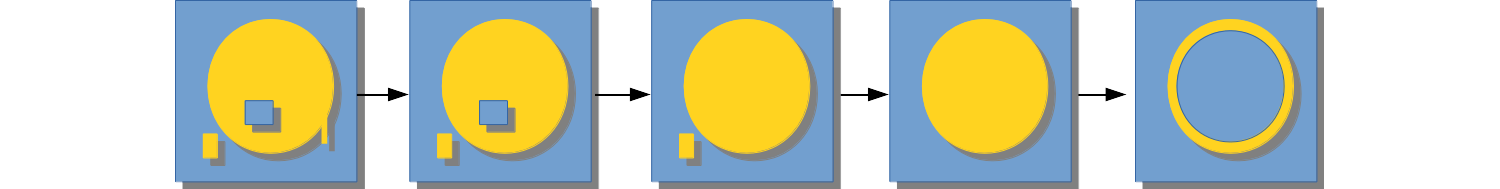
\includegraphics[width=18cm,trim=5cm 0cm 3cm 0cm, clip ]{contour.png}  
	\caption{Les étapes de la construction du volume. Les valeurs nulle sont présentées en bleu et les valeurs non nulle en orange. }
	\label{fig:lissage}
\end{figure} 

		\subsubsection{Construction de l'effet de volume}
	Pour avoir un effet de volume j'ai utilisé un algorithme simple. Il consiste a relié chaque point d'une surface par celui situé en face sur l'autre face. Pour résoudre le problème de la différence de taille, je relie certain point de la surface la plus petite à deux point de la surface la plus grande (\ref{fig:volumeMaillage}). Le nombre de points subissant cette opération est égale à la différence entre les deux surfaces. Pour savoir quand insérer un point supplémentaire, je divise la somme des points de la plus grandes surface par la différence. Par exemple, le nombre obtenu dans la figure \ref{fig:volumeMaillage} est de deux.

\vspace{0.25cm}
$  pas = nbrPtFace1 /(nbrPtFace2 - nbrPtFace2)$

\vspace{0.25cm}
La variable pas représente le nombre de point avant chaque insertion supplémentaire d'un point. nbrPtFace1 représente le nombre de point contenue par une face 1. Ce nombre est plus élevé que celui de la face 2. nbrPtFace2 représente le nombre de point contenue par une face 2.


\begin{figure}[h]
	\centering
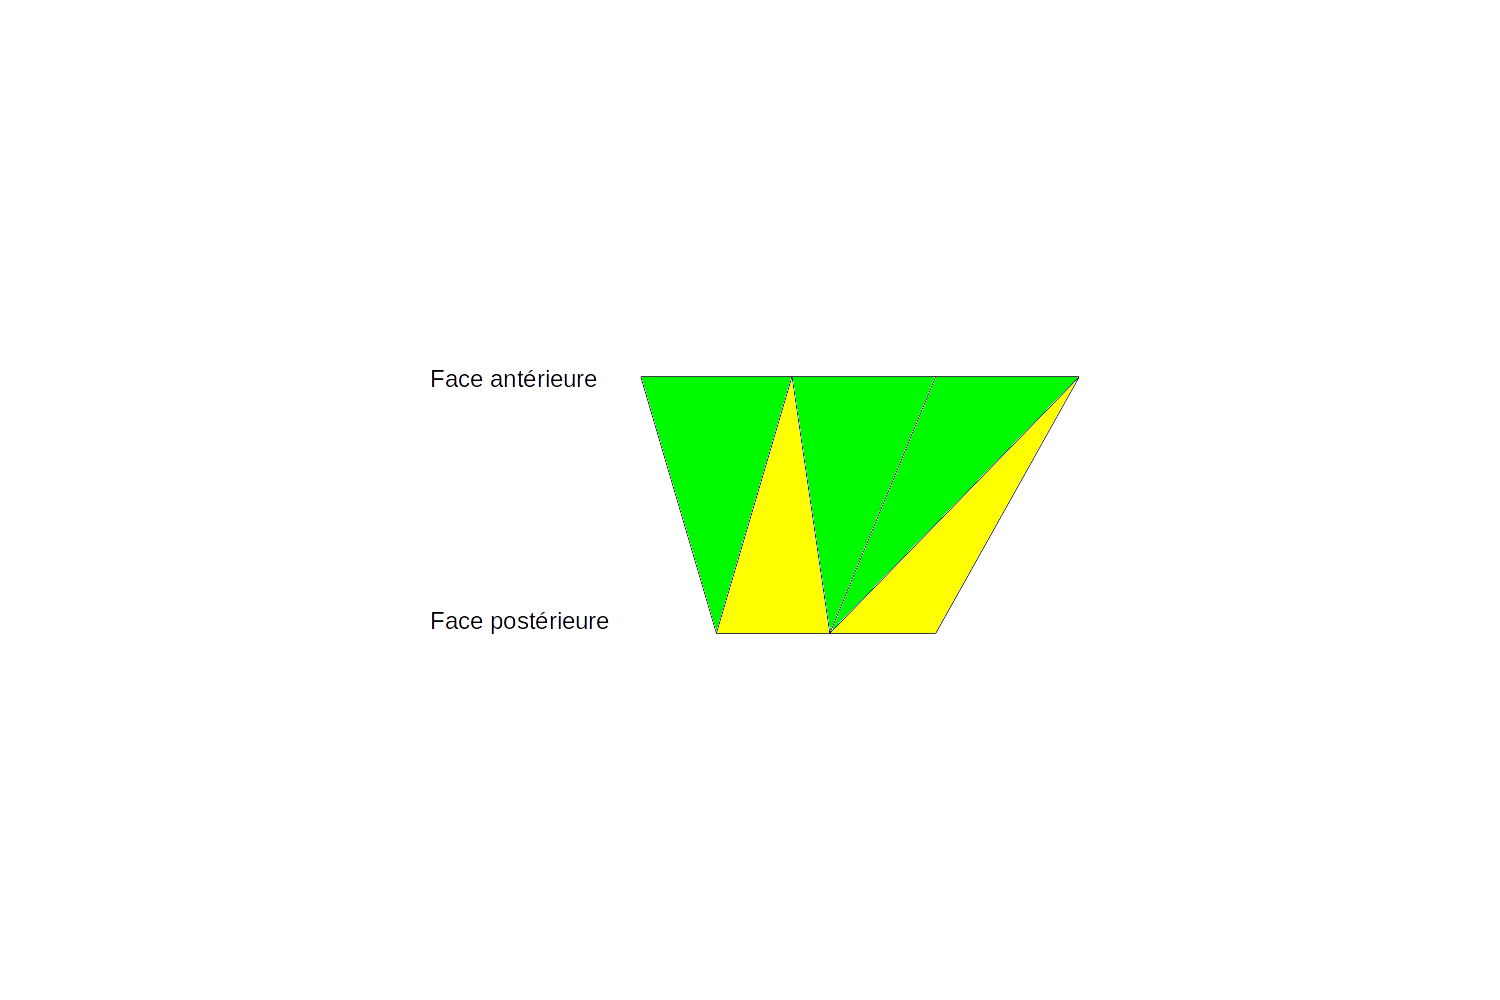
\includegraphics[width=15cm,trim=10cm 10cm 10cm 10cm, clip ]{volumeSchema.png} 
	\caption{Principe du maillage du volume.}
	\label{fig:volumeMaillage}
\end{figure} 

		\subsubsection{Visualisation}

Dans un premier temps, j'ai pu visualiser le volume (figure \ref{Volume}) seul puis associé aux faces antérieure et postérieure (figure \ref{resumeActor}) : 
\begin{figure}[h!]
	\centering
	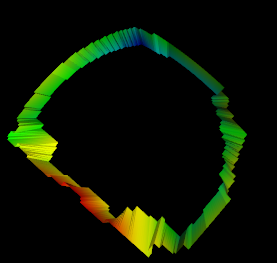
\includegraphics[width=8cm]{volume.png} 
	\caption{Affichage de l'effet de volume seul}
	\label{Volume}
\end{figure}
\begin{figure}[h!]
	\centering
	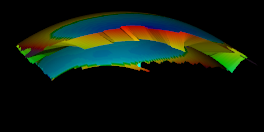
\includegraphics[width=10cm]{resumeActor.png} 
	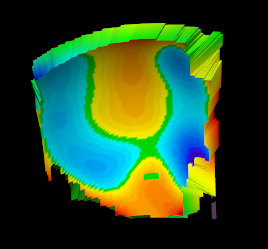
\includegraphics[width=10cm]{volume2.png} 
	\caption{Visualisation de la face antérieure et postérieure avec l'effet de volume}
	\label{resumeActor}
\end{figure}



%%%%%%%%%%%%%%%%%%%%%%%%% Programmation mobile %%%%%%%%%%%%%%%%%%%%%%%%%%%%%%%%%%S
\newpage
\section{VTK on Android}
	\subsection{Généralité sur la programmation mobile}

Il existe plusieurs systèmes d'exploitation permettant de faire fonctionner un appareil mobile tel que iOS, Android, Firefox OS, ou Windows Phone. Ces systèmes utilisent des langages et des outils différents. Par exemple, le système d'exploitation iOS fonctionne de préférence avec des applications en langage C, Objective-C ou HTML5, alors que le système d'exploitation Android fonctionne plutôt autour de Java. Certains langages multi-plateforme, tel que le C++, peuvent être utilisés aussi bien en Android qu'en iOS. 
	
	Pour faire de la visualisation en trois dimensions, les plateformes mobiles n'utilisent pas de l'OpenGL 2.0 ou 3.0  mais de l'OpenGL ES. C'est un dérivé de l'OpenGL adapté aux plateformes mobiles ou embarquées telles que les téléphones mobiles, les consoles de jeux vidéo portables... L'OpenGL ES possède une API plus légère en termes de mémoire et de coût de processeur, et une simplification plus poussée.
	
	La première étape afin de comprendre comment porter mon code en C++ sur Android a été d'étudier l'application Kiwiviewer. En effet, cette application  mobile fonctionne aussi bien sur Android que sur iOS et utilisant VTK.

	\subsection{VTK sur Android}
	Lorsque nous cherchons sur internet comment utiliser vtk sur Android, nous trouvons VES. VES est un framework open-source permettant la visualisation sur plateforme mobile. Il est constitué de deux librairies principales : VES et Kiwi. La librairie VES fournit les capacités et les infrastructures qui permettent la gestion des scènes en utilisant OpenGL ES. Kiwi est une librairie construite au-dessus de VES et de VTK afin de lier les deux. Kiwi est aussi divisée en plusieurs parties : celle qui permet de relier VES et VTK et deux autres spécifiques à Android ou iOS (figure \ref{kiwi}). Cette structure a été utilisée afin de construire le modèle Kiwiviewer. Le projet VES est accessible via gitHub, ce qui permet facilement d'installer, de voir les détails et les dates des mise à jours. 
	
\begin{figure}[h]
	\centering
	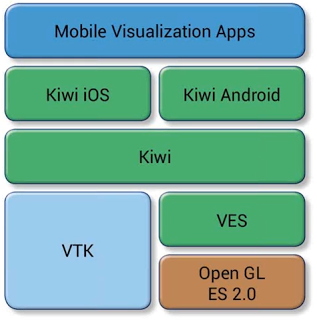
\includegraphics[width=5cm]{Kiwi.png} 
	\caption{Architecture d'une application mobile avec VTK et VES \cite{ndk538}}
	\label{kiwi}
\end{figure}


J'ai réussi à compiler VES mais il m'a été impossible de compiler la librairie Kiwi située dans VES, malgré le fait que je suivais le tutoriel point par point. Je ne trouvais pas un des fichiers permettant la compilation. La raison est que VES n'est plus maintenue. En effet, la dernière mise à jour date de juin 2014. De plus, Un article de Kitware informe que VES va \^etre déprécié en faveur de l'intégration d'un support pour iOS et Android dans VTK à partir de la mise à jour 6.2.0 de VTK \cite{ndk858, ndk860}.

L'installation pour Android de VTK se fait en deux étapes. La première est la compilation des outils de VTK. La deuxième est la compilation des outils ciblant l'architecture choisie d'Android. Cette deuxième compilation aura donc des options supplémentaires : le chemin menant au NDK, l'architecture d'Android (arm, X86, ...), le niveau de l'API et l'OpenGL ES version (2.0 ou 3.0).  

 	\subsection{NDK}
 Afin de permettre l'utilisation de C++ et de C sur Android, google a créé NDK. NDK (Kit de développement natif) est un outil permettant d'implémenter des parties natives (en C ou C++) dans les applications Android. Cela permet de créer du code commun (bibliothèque) entre plusieurs applications ou entre des applications Android et iOS par exemple\cite{ndk1}. VTK supporte les versions 5 à 10 de NDK. J'utilise donc la dernière versions qui est la 10e.
 
 \subsection{Environnement de Travail}
	Tout d'abord, afin de coder sur Android j'ai utilisé l'IDE Eclipse.  
 La première étape a été de trouver un IDE me permettant de construire une application Android. Les choix qui se présentaient à moi étaient : Eclipse et Android studio.
 
 	\subsubsection{Eclipse}
 Le premier IDE que j'ai utilisé a été Éclipse. En effet, la page officiel de NDK \cite{ndk2} utilise Éclipse pour son tutoriel et de nombreux tutoriels l'utilisent.Afin d'utiliser Android sur Eclipse il est nécessaire d'installer l'ADT (Android Development Tools). Deux fichiers sont utilisés afin de pouvoir utiliser du C ou du C++ en plus du NDK : Android.mk et Application.mk. Il est aussi nécessaire d'installer ant.
 
 En me renseignant un peu plus il s'est avéré que google ne supporterait plus ADT afin de se concentrer uniquement sur un IDE spécifique au développement Android : Android Studio. Je suis passé uniquement sur Android Studio.
 
 	\subsubsection{Android Studio}
 	Pour fonctionner, Android Studio utilise plusieurs systèmes dont Gradle. De plus, un dossier appelé "jni" doit exister lors de l'introduction de code en C ou C++. 
\paragraph{Gradle} est un moteur de production fonctionnant sur la plateforme Java. Il permet de construire des projets en Java, Scala, Groovy voir C++. Il possède plusieurs fichiers script de configuration : 
 	
 	\begin{enumerate}
 	\item gradle-wrapper.propertie : C'est le script par lequel la compilation commence. Il permet de vérifier la version de gradle et de télécharger la version voulue.
 	\item local.property : permet de définir les chemins absolus du SDK et du NDK.  
 	\item setting.gradle : Déclare la configuration requise pour installer et configurer la hiérarchie des instances d'un projet qui participe lors de la compilation.
 	\item build.gradle (Projet) : permet de définir les options communes à tous les sous-projet et modules.
 	\item build.gradle (module: app) : permet de définir les options spécifiques au projet.
 	\end{enumerate}

\paragraph{JNI} est un dossier contenant la partie native du code (C, C++).
\vspace{0.25cm}

 	Dans de mes premiers tests, j'ai utilisé une partie du système d'Eclipse. C'est à dire, que mon code contient les fichiers Android.mk et Application.mk. Mais des réglages de Gradle sont nécessaire afin de permettre l'utilisation de C et de C++. Tout d'abord, il doit conna\^itre le chemin absolu du NDK, puis la version de Gradle ainsi que son plugin. Ensuite, il a besoin du niveau de l'API utilisé ainsi que tout les réglages liés au C ou C++. Avec ce test j'ai réussi à compiler et à afficher un "Hello World" sur le simulateur en API 21 en utilisant du C, mais je n'ai pas réussi avec du C++.
 	
 	Par la suite, google a sorti la version 1.3 de Android Studio. A partir de cette version il est possible de coder en C++ sur Android Studio. J'ai pu compiler un de leur exemples et ainsi étudier comment il fonctionne.

\parindent=0.0em
\textbf{Plugin de Gradle: } version expérimentale, c'est à dire la 0.2.0 (build.gradle (Projet)).

\textbf{Version de Gradle : } 2.5. J'ai essayé la 2.4 et l'exemple ne compile pas (gradle-wrapper.propertie).

\textbf{build.gradle (Module:app) : }  Au lieu d'utiliser "com.Android.application" pour spécifier que c'est une application ils utilisent "com.Android.model.application". De plus, une fonction qui s'appelle model a été rajoutée. Ces deux éléments sont spécifique au plugin expérimental de Gradel. Dans la fonction model, nous allons trouver la fonction Android permettant de configurer la version de SDK, de l'API, des outils de compilation, et le chemin pour accéder au projet. Nous trouvons aussi Android.ndk, une fonction permettant de configurer la ndk du projet (nom du projet, chemins des librairies, des includes, la librairie de C++).

\parindent=1.5em

En utilisant NativeActivity ("public class MoreTeapotsNativeActivity extends NativeActivity"), Android peut être complètement codé en C++. Dans ces conditions, la fonction main est remplacée par Android-main. Android-main devra donc assumer les fonctions occupées normalement par un main de C++ et celui d'Android.  Bien s\^ur certaines fonctions peuvent \^etre codées en java et \^etre transmises au code C++ gr\^ace à des fonctions liant les deux. Ainsi sur l'exemple de moreTeapot le nombre de FPS a pu \^etre ajouté. Des fonctions contenues dans le dossier cpu-feature permettent de remplacer les fonctions utilisées qui auraient d\^u \^etre utilisées en Java afin d'assumer l'événementiel, la visualisation et autre... 

	\subsection{VTK et Android Studio}
	
	Après avoir étudié les tests, je suis passé au test sur VTK. J'ai donc pris un exemple de VTK disponible pour Android. Cet exemple était à l'origine fait pour un projet fait sous éclipse, donc qui n'utilise pas gradle. J'ai donc rencontré certains problèmes. 
	
	Le premier problème a été qu'Android Studio ne trouvait pas les "includes" utilisés par l'exemple de VTK. Il a donc été nécessaire de lui spécifier les chemins de ces "includes". Ces chemins sont ajoutés à des CPPFlags.
	
	Le deuxième problème a été la librairie utilisée pour C++. En effet, la librairie utilisée par l'exemple moreTeapots était la	 "stlport\_static", or elle ne reconnait pas certains objets de VTK tels que le vtktype. Pour corriger ce problème j'ai utilisé la bibliothèque "gnustl\_static". Pour spécifier la librairie, j'ai inséré le nom de la librairie dans la variable stl.
	
	Le troisième problème était un défaut sur les exceptions sur les rtti ("error: cannot use typeid with -fno-rtti"). Elle a été corrigée en ajoutant dans la variable CPPFlags l'option "-frtti".
	
	Le quatrième problème était que le compilateur n'acceptait pas quand du code était mis dans les "header" et cela même en utilisant la fonction "inline" permettant normalement de palier le problème. L'erreur qui s'affiche indique qu'il ne trouve pas certaines classes où se situe les headers avec le code (Exemple de cette erreur : "undefined reference to `vtkRenderWindow::New()'"). La première solution que j'ai trouvé a été de réécrire ces classes afin que le code contenu dans les "header" soit mis dans les fichiers source. Cela a marché et les erreurs disparaissaient mais j'ai trouvé une autre solution qui consiste à spécifier la version du compilateur. Ici la version que j'ai utilisé est la c++11 en spécifiant dans un CPPFlags "-std=c++11". Cela a fonctionné mais la m\^eme erreur c'est présentée dans l'exemple donné par VTK. Il n'a pas été possible de trouver de solutions pour aller plus loin.

%%%%%%%%%%%%%%%%%%%%%%%%% Discution %%%%%%%%%%%%%%%%%%%%%%%%%%%%%%

\newpage
\section{Discussion}
	 \subsection{Environnement de développement}
J'ai préféré utiliser l'association entre Sublime text et CMAKE plut\^ot que l'utilisation d'un IDE tel que code::block. En effet, les exemples de VTK utilisaient déjà CMAKE donc leur "CMAKELists.txt" ont pu me servir de base à la construction de celui de mon projet. De plus, étant débutant en C++ j'ai trouvé que cette manière de faire me permettais de mieux comprendre la construction d'un projet en C++. Je trouve aussi qu'il est important de comprendre CMAKE pour des projets future.

	\subsection{Difficulté de la programmation mobile}
	 Séduit par cette application, je l'ai étudié dans l'espoir de pouvoir y baser ma propre application. Malheureusement, cette application n'était plus mise à jours régulièrement. En effet, VTK a décidé d'arrêter son développement afin d'inclure la partie Android et iOS dans VTK en lui même. Au même moment, à environ un mois de décalage, google décide d'arrêter la mise à jours d'ADT pour éclipse et de passer uniquement sur Android Studio. Du fait de ces deux évènements peu de documentation était disponible. En effet, il existait peu de tutoriels pour utiliser VTK sur Android et aucun sur Android Studio. Les exemples fournis par VTK ont été fait sur Eclipse.
	 
%%%%%%%%%%%%%%%%%%%%%%%%% Conclusion %%%%%%%%%%%%%%%%%%%%%%%%%%%%%%%
\newpage
\section{Conclusion}
Lors de ce stage, j'ai pu visualiser une cornée en trois dimensions via une bibliothèque en C++ appelée VTK ou Visual Tool Kit, et j'ai commencer les étapes pour la visualiser sur une plateforme mobile Android mais cela reste à finir. La visualisation de la cornée m'a permis de beaucoup apprendre sur la programmation orientée objet avec le langage C++ et sur la visualisation en trois dimension. Avec C++, j'ai aussi appris à utiliser CMAKE, un logiciel que j'avais déjà vu lors de ma formation précédente mais sans comprendre comment il fonctionnait. J'ai aussi pu approfondir ma pratique dans la manipulation des pointeurs et dans la création de template. Même s'il ne m'a pas été possible de compiler l'exemple de VTK sur Android, mes recherches m'ont permis d'en apprendre beaucoup sur Android et notamment sur la partie C++ (NDK) qui n'est pas la plus simple.


  VTK est un très bon outils pour la visualisation. Une fois pris en main, j'ai pu aisément afficher la cornée ainsi que les couleurs correspondant à la vrai palette utilisé par les praticien. Mais VTK ne se limite pas seulement à la visualisation, il permet aussi d'interagir avec l'objet en le bougeant, l'agrandissant ou le diminuant. Il est aussi possible d'augmenter sa largeur ou sa hauteur. Il pourrais donc \^etre intéressant d'ajouter ce genre d'interaction. Pour le côté Android, il faudrait réussir à compiler VTK sur Android et de contacter KITWARE, dont fait partie VTK, pour demander de l'aide si ce n'est pas possible.

%%%%%%%%%%%%%%%%%%%%%%%%% Référence %%%%%%%%%%%%%%%%%%%%%%%%%%%%%%%%
\newpage

\bibliographystyle{plain} % Le style est mis entre accolades.
\bibliography{biblio}



\end{document}


